%文档命令 texdoc tikz
\documentclass{article}
\usepackage{lipsum}
\usepackage{amsmath, mathrsfs, amsfonts}
\usepackage{tikz}
\usepackage{graphicx}
\usetikzlibrary{patterns} %使用 tikz 的库

% cyan 青色;magenta 洋红


\begin{document}
    \centering
    Hello world!
    \[ a^2 + b^2 = c^2 + d^2 \]
    Goodbye.

%画直线
    \begin{figure}[htbp]
        \centering
        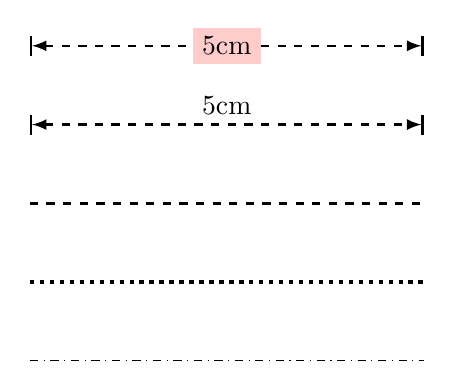
\begin{tikzpicture}[>=latex]  % 放在 begin 后边的是宏操作;箭头类型还有 stealth
            \draw[|<->|, dashed, thick] (0, 0)--node[above]{5cm}(5, 0);
            % node 结点 ,above, below, right, left, "=3mm":调整结点位置
            % node 在谁的后边,图上结点就在对应的位置
            
            \draw[|<->|, dashed, thick] (0, 1)--node[fill = red!20!white]{5cm}(5, 1);
            % xcolor 的宏包可以实现颜色调配;"red!20!white" 是百分之20的红色加上百分之80的白色
            
            \draw[dashed, very thick] (0, -1) to (5, -1);
            \draw[dotted, ultra thick] (0, -2) to (5, -2);
            \draw[dashdotted, thin] (0, -3) to (5, -3);
        \end{tikzpicture}
        \caption{}
    \end{figure}

%画坐标
    \begin{figure}[htbp]
        \centering
        \begin{tikzpicture}[>=latex]
            \draw[->] (-1, 0) -- (4, 0)node[below]{$x$};
            \draw[->] (0, -1) -- (0, 4)node[left]{$y$};
            \draw (0, 2)node[left]{$N$} -- (2, 2)node[right]{$P(x,y)$} -- (2, 0)node[below]{$M$};
            \node at (-.2, -.2){$O$};   %"\node at" 在某一点写入文本
            \draw (1, 0)node[below]{$1$} -- (1, .1);
            \draw (0, 1)node[left ]{$1$} -- (.1, 1);

        \end{tikzpicture}
        \caption{}
    \end{figure}

%画坐标
    \begin{figure}[htbp]
        \centering
        \begin{tikzpicture}[>=latex]
            \draw[->] (-1, 0) -- (4, 0)node[below]{$x$};
            \draw[->] (0, -1) -- (0, 4)node[left ]{$y$};
            \foreach \c in {1, 2, 3}
            {
                \draw[thick] (0, \c)node[left ]{$\c$} -- (.1, \c);
                \draw[thick] (\c, 0)node[below]{$\c$} -- (\c, .1);
                \foreach \b in {1, 2, ..., 9}
                {
                    \draw[thin] (0, \c - \b*0.1) -- (.05, \c - \b*0.1);
                    \draw[thin] (\c - \b*0.1, 0) -- (\c - \b*0.1, .05);
                }
            }
        \end{tikzpicture}
        \caption{}    
    \end{figure}

%填充
    \begin{figure}[htbp]
        \centering
        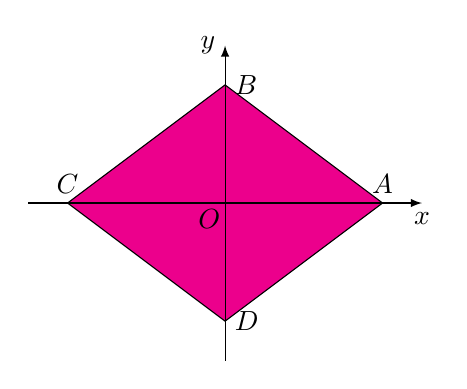
\begin{tikzpicture}[>=latex, scale=.5] %scale 用来缩放图像,文字大小不变
            \draw[fill=magenta] (0, 3)node[right]{$B$} -- (4, 0)node[above]{$A$} -- (0, -3)node[right]{$D$} -- (-4, 0)node[above]{$C$} -- (0, 3);
            %fill = colors 直接填充会覆盖
            %解决:将填充的代码行提前,调整顺序
            \draw[->] (-5, 0) -- (5, 0)node[below]{$x$};
            \draw[->] (0, -4) -- (0, 4)node[left]{$y$};
            \node at (-.4, -.4){$O$};   %"\node at" 在某一点写入文本
        \end{tikzpicture}
        \caption{}
    \end{figure}

%rectangle, circle, arc 画图
    \begin{figure}[htbp]
        \centering
        \begin{tikzpicture}[>=latex]
            %\draw[fill=cyan] (0, 0) rectangle (4, 3);
            %\fill [cyan, draw=black] (0, 0) rectangle (4, 3); 效果与上一句完全相同
            %rectangle 用来画矩形
            %draw[fill=color] 会留下边框,去除边框可以用\fill
            %\fill [cyan] (0, 0) rectangle (4, 3);
            %(圆心坐标)circle(半径) 圆形
            %极坐标 (theta:rho) ,其中 theta 是角度,不是弧度
            \draw (0, 0) -- (4, 0);
            \draw (0, 0) -- (45:4);
            \draw[->] (.5, 0) arc (0: 45: .5);
            %(起始点坐标) arc (起始角度: 旋转角度: 半径)



        \end{tikzpicture}
        \caption{}
    \end{figure}

%练习一
    \begin{figure}[htbp]
        \centering
        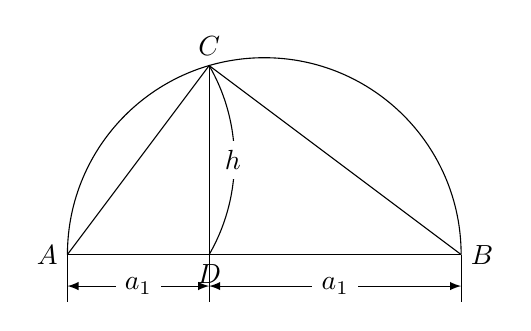
\begin{tikzpicture}[>=latex]
            % \draw (0, 0)node[left]{$A$} -- (4, 0)node[right]{$B$};
            % \draw[|<->|] (0, -.1) -- (4, -.1);
            % \draw (4, 0) arc (0: 180: 2);
            % \draw (0, 0) -- (60: 2)node[above]{$C$} -- (4, 0);
            % \draw (60: 2) -- (1, 0)node[below]{$D$};
            \draw (0,0)node[left]{$A$}--(5,0)node[right]{$B$};
            \draw (0,0) arc (180:0:2.5);
            \draw (1.8,2.4)node[above]{$C$}--(1.8,0)node[below]{$D$};
            \draw (0,0)--(1.8,2.4)--(5,0);
            \draw[<->] (0,-.4)--node[fill=white]{$a_1$}(1.8,-.4);
            \draw[<->] (1.8,-.4)--node[fill=white]{$a_1$}(5,-.4);
            \draw (0,0)--(0,-.6);
            \draw (1.8,0)--(1.8,-.6);
            \draw (5,0)--(5,-.6);
            \draw (1.8,0) arc (-30:30:2.4);
            \node[fill=white] at (2.1,1.2) {$h$};

            
        \end{tikzpicture}
        \caption{}
    \end{figure}

%练习二
    \begin{figure}[htbp]
        \centering
        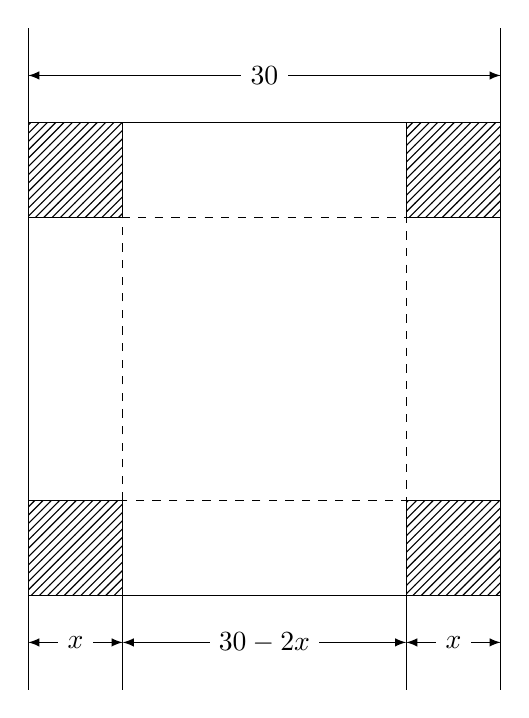
\begin{tikzpicture}[>=latex,scale=.6]
            \draw (0, 0) rectangle (10, 10);
            \draw[dashed] (2, 2) rectangle (8, 8);
            \draw[pattern = north east lines] (0, 0) rectangle (2, 2);
            \draw[pattern = north east lines] (8, 0) rectangle (10, 2);
            \draw[pattern = north east lines] (0, 8) rectangle (2, 10);
            \draw[pattern = north east lines] (8, 8) rectangle (10, 10);
            \foreach \x in {0, 2, 8, 10}
            {
                \draw (\x, 0) -- (\x, -2);
            }
            \draw[<->] (0, -1) --node[fill=white]{$x$} (2, -1);
            \draw[<->] (2, -1) --node[fill=white]{$30-2x$} (8, -1);
            \draw[<->] (8, -1) --node[fill=white]{$x$} (10, -1);
            \foreach \x in {0, 10}
            {
                \draw (\x, 10) -- (\x, 12);
            }
            \draw[<->] (0, 11) --node[fill=white]{$30$} (10, 11);
        \end{tikzpicture}
        \caption{}
    \end{figure}

    \begin{figure}[htbp]
        \centering
        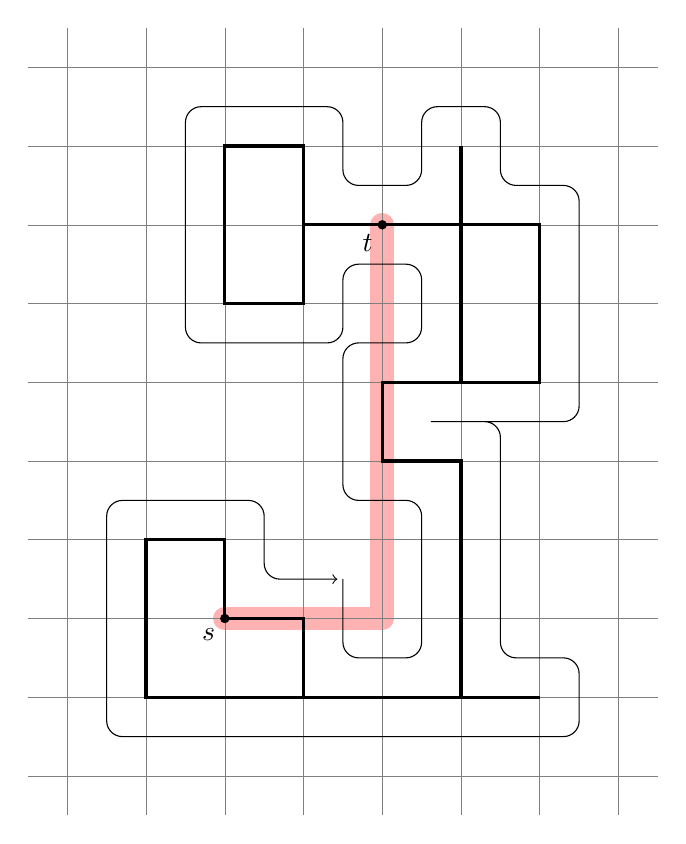
\begin{tikzpicture}
            \draw[line width=0.3cm,color=red!30,line cap=round,line join=round] (0,0)--(2,0)--(2,5);
            \draw[help lines] (-2.5,-2.5) grid (5.5,7.5);
            \draw[very thick] (1,-1)--(-1,-1)--(-1,1)--(0,1)--(0,0)--
            (1,0)--(1,-1)--(3,-1)--(3,2)--(2,2)--(2,3)--(3,3)--
            (3,5)--(1,5)--(1,4)--(0,4)--(0,6)--(1,6)--(1,5)
            (3,3)--(4,3)--(4,5)--(3,5)--(3,6)
            (3,-1)--(4,-1);
            \draw[below left] (0,0) node(s){$s$};
            \draw[below left] (2,5) node(t){$t$};
            \fill (0,0) circle (0.06cm) (2,5) circle (0.06cm);
            \draw[->,rounded corners=0.2cm,shorten >=2pt]
            (1.5,0.5)-- ++(0,-1)-- ++(1,0)-- ++(0,2)-- ++(-1,0)-- ++(0,2)-- ++(1,0)--
            ++(0,1)-- ++(-1,0)-- ++(0,-1)-- ++(-2,0)-- ++(0,3)-- ++(2,0)-- ++(0,-1)--
            ++(1,0)-- ++(0,1)-- ++(1,0)-- ++(0,-1)-- ++(1,0)-- ++(0,-3)-- ++(-2,0)--
            ++(1,0)-- ++(0,-3)-- ++(1,0)-- ++(0,-1)-- ++(-6,0)-- ++(0,3)-- ++(2,0)--
            ++(0,-1)-- ++(1,0);
        \end{tikzpicture}
    \end{figure}


    
\end{document}